% ---------------------------------------------------------------------------
% Author guideline and sample document for EG publication using LaTeX2e input
% D.Fellner, v1.13, Jul 31, 2008

\documentclass{egpubl}
\usepackage{eg2014}

% --- for  Annual CONFERENCE
%\ConferenceSubmission   % uncomment for Conference submission
% \ConferencePaper        % uncomment for (final) Conference Paper
% \STAR                   % uncomment for STAR contribution
% \Tutorial               % uncomment for Tutorial contribution
% \ShortPresentation      % uncomment for (final) Short Conference Presentation
% \Areas                  % uncomment for Areas contribution
% \MedicalPrize           % uncomment for Medical Prize contribution
% \Education              % uncomment for Education contribution
%
% --- for  CGF Journal
%\JournalSubmission    % uncomment for submission to Computer Graphics Forum
\JournalPaper         % uncomment for final version of Journal Paper
%
% --- for  CGF Journal: special issue
% \SpecialIssueSubmission    % uncomment for submission to Computer Graphics Forum, special issue
% \SpecialIssuePaper         % uncomment for final version of Journal Paper, special issue
%
% --- for  EG Workshop Proceedings
% \WsSubmission    % uncomment for submission to EG Workshop
% \WsPaper         % uncomment for final version of EG Workshop contribution
%
 \electronicVersion % can be used both for the printed and electronic version

% !! *please* don't change anything above
% !! unless you REALLY know what you are doing
% ------------------------------------------------------------------------

% for including postscript figures
% mind: package option 'draft' will replace PS figure by a filname within a frame
\ifpdf \usepackage[pdftex]{graphicx} \pdfcompresslevel=9
\else \usepackage[dvips]{graphicx} \fi

\PrintedOrElectronic

% prepare for electronic version of your document
\usepackage{t1enc,dfadobe}

\usepackage{egweblnk}
\usepackage{cite}

% For backwards compatibility to old LaTeX type font selection.
% Uncomment if your document adheres to LaTeX2e recommendations.
% \let\rm=\rmfamily    \let\sf=\sffamily    \let\tt=\ttfamily
% \let\it=\itshape     \let\sl=\slshape     \let\sc=\scshape
% \let\bf=\bfseries

% end of prologue



\usepackage[usenames,dvipsnames,svgnames]{xcolor}
\usepackage{enumitem}
\usepackage{subcaption}
\usepackage{flushend}
\usepackage{multirow}
\usepackage{booktabs}
\usepackage{tikz}
\usepackage{relsize}
\usepackage{algorithm2e}


\makeatletter
\newcommand{\removelatexerror}{\let\@latex@error\@gobble}
\makeatother

%% define colors for algorithm
%\definecolor{algoColorKeyword}{named}{blue}
%\definecolor{algoColorComment}{named}{olive}

%% setup for algorithms
\SetAlgoInsideSkip{}
\SetAlgoLined
\SetCommentSty{emph}


\def\etal{\emph{et al.}}
\setlength{\fboxsep}{0pt}
\newcommand{\red}[1]{{\color{red}#1}}
\newcommand{\yellow}[1]{{\color{Goldenrod}#1}}
\newcommand{\green}[1]{{\color{PineGreen}#1}}
\newcommand{\minor}[1]{\yellow{#1}}
\newcommand{\new}[1]{\green{#1}}
\newcommand{\todo}[1]{{\color{red}\emph{(#1)}}}
\newcommand{\remark}[1]{{\color{blue!80!white}\textbf{Remark:} #1}}
\newcommand{\bin}[1]{b^{#1}}
\newcommand{\dbin}[2]{b^{#1-#2}}
\newcommand{\code}[1]{\texttt{#1}}
\newcommand{\POne}{Problem 1}
\newcommand{\PTwo}{Problem 2}
\newcommand{\ab}{\mbox{A-buffer}}
\newcommand{\dc}{DC}
\newcommand{\dch}{DCH}
\newcommand{\dci}{DCI}
\newcommand{\stencil}{ppAO}
\newcommand{\dloop}{ppDP}

\newlength{\imgWidth}
\setlength{\imgWidth}{0.23\textwidth}
\newlength{\boxheight}
\newsavebox{\savedProteinBox}
\newif\ifSplitBoxFramed
\newcommand{\enableSplitImgFrame}{\SplitBoxFramedtrue}
\newcommand{\disableSplitImgFrame}{\SplitBoxFramedfalse}
\enableSplitImgFrame

%% split two images (param 1, param 2)  along a diagonal line
\newcommand{\splitImage}[2]{%
  \begin{tikzpicture}[x=\imgWidth,y=-\imgWidth] %% gives us a figure in coordinates [0:0] to [1:1]
    \clip (0,0) rectangle (1,1);
    %% full color picture (left)
    \begin{scope}[]
      \clip (0,0) -- (\topLineRatio,0) -- (\bottomLineRatio,1) -- (0,1);
      \draw(0,0) node[anchor=north west,inner sep=0pt]{%
        \includegraphics[width=\imgWidth]{#1}};
    \end{scope}
    %% depth complexity (right)
    \begin{scope}[]
      \clip  (\topLineRatio,0) -- (\bottomLineRatio,1) -- (1,1) -- (1,0);
      \draw(0,0) node[anchor=north west,inner sep=0pt]{%
        \includegraphics[width=\imgWidth]{#2}};
    \end{scope}
    %% separation line
    \draw[black,very thick] (\topLineRatio,0) -- (\bottomLineRatio,1) ;
    \ifSplitBoxFramed%
      %% frame box
      \draw[line width=1pt] (0,0) rectangle (1,1);
    \fi
  \end{tikzpicture}
}


%% define golden ratio
\newcommand{\goldenRatioLong}{0.618}
\newcommand{\goldenRatioShort}{0.382}

%% sets the line start and end points for splitting images along the vertical axis
%% arg1 sets the point on the top line
%% arg2 sets the point on the bottom line
\newcommand{\setSplitLineRatios}[2]{%
  \def\topLineRatio{#1}
  \def\bottomLineRatio{#2}
}


% ---------------------------------------------------------------------
% EG author guidelines plus sample file for EG publication using LaTeX2e input
% D.Fellner, v1.17, Sep 23, 2010

%% original Eurographics Title
\title[Hybrid Data Visualization]%
      {Hybrid Data Visualization\\Based On Depth Complexity Histogram Analysis}

% % for anonymous conference submission please enter your SUBMISSION ID
% % instead of the author's name (and leave the affiliation blank) !!

% %% Full author first names
% \def\SL{Stefan Lindholm}
% \def\MF{Martin Falk}
% \def\ES{Erik Sund\'en}
% \def\AB{Alexander Bock}
% \def\AY{Anders Ynnerman}
% \def\TR{Timo Ropinski}
%% Abbreved author first names
\def\SL{S.~Lindholm}
\def\MF{M.~Falk}
\def\ES{E.~Sund\'en}
\def\AB{A.~Bock}
\def\AY{A.~Ynnerman}
\def\TR{T.~Ropinski}

%%% Author and Affiliation (multiple authors with single affiliations).
 %\author[S.~Lindholm et al.]{%
		%\SL \thanks{e-mail: stefan.lindholm@liu.se},%
		%\MF, \ES, \AB, \AY,%
		%and \TR \thanks{e-mail: timo.ropinski@liu.se}\\%
		%Scientific Visualization Group, 
		%Department of Science and Technology, 
		%Link{\"o}ping University}

%% Emails below author names
\author[S.~Lindholm et al.]%
		{\SL, \MF, \ES, \AB, \AY, and \TR\\% 
		Scientific Visualization Group, 
		Department of Science and Technology, 
		Link{\"o}ping University\\% 
		\{stefan.lindholm$|$timo.ropinski\}@liu.se}

%\author[CGF-14-EG-016.R1]
       %{CGF-14-EG-016.R1}

% ------------------------------------------------------------------------

% if the Editors-in-Chief have given you the data, you may uncomment
% the following five lines and insert it here
%
% \volume{27}   % the volume in which the issue will be published;
% \issue{1}     % the issue number of the publication
% \pStartPage{1}      % set starting page


%-------------------------------------------------------------------------
\begin{document}

\setSplitLineRatios{\goldenRatioLong}{\goldenRatioShort}

%\teaser{\centering
%  \splitImage{snapshots/mol/mol-zoom_1024}{snapshots/mol/mol-zoom_dci-norm-inv}
%  \hfill
%  \splitImage{snapshots/dti/dti5}{snapshots/dti/dti5_dci-norm-inv}
%  \hfill
%  \splitImage{snapshots/space/space}{snapshots/space/space_dci-inv}
%  \hfill
%  \splitImage{snapshots/flow/test_flow_white}{snapshots/flow/test_flow_dci-norm-inv}
%  %
%  \caption{\label{fig:teaser}
%    %% new caption
%    Our rendering algorithm applied to proteins, diffusion tensor imaging fibers, coronal mass ejections of the sun, and flow data (left to right) showing the final result and the depth complexity. The algorithm is optimized for hybrid data, including both semi-transparent volumetric and geometric sources.
%    % The left parts show the final result and the right parts depict the depth complexity.
%  }
%}

\maketitle

\begin{abstract}
%
In many cases, only the combination of geometric and volumetric data sets is able to describe a single phenomenon under observation when visualizing large and complex data.
%% Problem: 1. transparent geometry, requires sorting, 2. fusing/combining volume rendering with the geometry
When semi-transparent geometry is present, correct rendering results require sorting of transparent structures. 
Additional complexity is introduced as the contributions from volumetric data have to be partitioned according to the geometric objects in the scene.
%% Solution: (already known)
The \ab{}, an enhanced framebuffer with additional per-pixel information, has previously been introduced to deal with the complexity caused by transparent objects. 
%% our stuff/contribution:
In this paper, we present an optimized rendering algorithm for hybrid volume-geometry data based on the \ab{} concept. 
We propose two novel components for modern GPUs that tailor memory utilization to the depth complexity of individual pixels.
The proposed components are compatible with modern \ab{} implementations and yield performance gains of up to eight times compared to existing approaches through reduced allocation and reuse of fast cache memory. 
%
We demonstrate the applicability of our approach and its performance with several examples from molecular biology, space weather, and medical visualization containing both, volumetric data and geometric structures.

\begin{classification} % according to http://www.acm.org/class/1998/
\CCScat{Computer Graphics}{I.3.3}{Picture/Image Generation}{Display algorithms}
\CCScat{Computer Graphics}{I.3.7}{Three-Dimensional Graphics and Realism}{}
\CCScat{Computer Graphics}{I.3.8}{Applications}{}
\end{classification}

\end{abstract}


%-------------------------------------------------------------------------
\section{Introduction}
\label{sec:introduction}

With the widespread use of imaging technologies in data intensive research fields, visualization becomes an enabling technology that supports the exploration of acquired data sets. 
A recent trend is the multitude of data that arise not only in the form of multimodal volumetric data sets but also from geometric representations, which may be derived from the data or are acquired in different ways.
Consequently, a challenge in visualization research is the efficiency and effectiveness at which this hybrid data can be rendered in a single setting. 
In many cases the integrated geometry is of similar or higher complexity than the volumetric data with which it should be combined. 
While modern volume rendering supports the inspection of otherwise dense data sets by facilitating semi-transparency, additional challenges arise when multiple volumes are combined with geometric data. 
Recent work suggests that geometric representations also benefit from semi-transparent properties~\cite{Guenther:2013:TOG}. 
Nevertheless, current state-of-the-art algorithms cannot always deliver interactive exploration for complex and semi-transparent hybrid data. 
Interactivity is, however, an essential feature when exploring scientific data sets.

In this paper, we improve upon existing techniques to facilitate efficient visualization of hybrid data sets as they occur in today's imaging-dependent areas of science. 
The fundamental challenge, arising when blending multiple semi-transparent sources into a single image, is to ensure that the elements are blended in view-dependent front-to-back or back-to-front order. 
When fusing multiple volumes or including mesh geometry into the visualization pipeline, the sorting must be ensured along each viewing ray.
This results in a performance bottleneck as well as in increased memory usage. 
As these shortcomings hinder interactive exploration of many hybrid data sets, we have analyzed several of these data sets from different real-world scenarios with the goal to develop an optimized rendering algorithm enabling interactive exploration. 
As a tool in the analysis we have used {Depth Complexity Histograms} (\dch) that correspond to the observed depth complexity across all pixels in the rendered image for a given scene and camera setting. 
The \dch{}s have been used to identify trends in the global distribution for scenes with hybrid data and to determine how these trends relate to rendering complexity. 
%% Technical
Based on the similarities of the occurring distributions, we propose two novel components which we combine with existing techniques to form an optimized rendering algorithm for hybrid data. 
The first component minimizes the allocated size in fast cache memory by adjusting the allocation to pixel depth complexity. 
The second component partitions the depth sorting similarly to depth peeling and recycles a smaller amount of allocated memory. 
As a result, computational throughput is increased and the maximum supported depth complexity is less dependent on the amount of available local GPU memory. 
The components provide between three and eightfold performance increase compared to existing algorithms. 
These qualities enable the interactive visualization of large and complex hybrid data sets at interactive frame rates, which is one of the key ingredients for enabling scientific discoveries in data-intense sciences.



\section{Related Work}
\label{sec:related-work}

\noindent\textbf{Data fusion.} 
%
One aspect of hybrid data rendering relates to fusion of multiple volumetric sources.
Several publications have investigated how samples from multiple sources should be blended, including different levels of intermixing~\cite{cai99intermixing}. 
A recent comparison of different intermixing schemes was presented by Schubert and Scholl~\cite{Schubert2011}. 

Rendering multiple volumes with arbitrary placement, orientation, and resolution is often associated with computational costs for scene partitioning. 
To limit the per frame rendering cost, object space is often separated into convex regions homogeneously occupied by a fixed number of volumes. 
The convex regions are then sorted, either using specialized data structures~\cite{grimm04vobjects,lindholm2009fused,Lux2009} or using depth peeling techniques~\cite{Plate2007,rossler08multishader}. 
Many of these approaches also utilize shader instantiation, similar to one of the components presented in this paper, but do not include solutions for inclusion of semi-transparent geometry. 

Fusing opaque geometry with volumetric data is straightforward in most volume rendering pipelines and does not require a full scene partition~\cite{engel2006volume}. 
Semi-transparent geometry, on the other hand, is more computationally demanding as the resulting object space partitioning is costly, particularly if the geometry is not closed or has concave features. 
Image space techniques have been used in such situations as these techniques are generally well adapted to inclusion of generic, semi-transparent geometry \cite{brecheisen08multimodal,kainz2009ray}. 
With these methods, entry and exit points for homogeneously occupied ray segments are extracted from the volume proxy geometry and scene partitioning is performed on a per-ray basis during rasterization.
The advantages and disadvantages of the available image space approaches are directly related to which transparency technique they employ, i.e. depth peeling and \ab{}s, which are discussed below. 


\noindent\textbf{Transparency rendering.}
%
To ensure correct blending order of multiple semi-transparent samples, Order Independent Transparency (OIT) algorithms have been an ongoing research topic for the last thirty years~\cite{Maule2011}. 
Two of the most widespread approaches are depth peeling and \ab{}s. 
Our algorithm follows the principles and global memory management of the \ab{}, which yields superior performance for scenes with high depth complexity \cite{Yang2010,Kauker2013}. 

The \ab{} is a leading OIT solution based on the temporary storage and sorting of intermediate pixel fragments. 
The concept was first introduced by Carpenter~\cite{Carpenter1984}. 
Subsequent works improved the concept~\cite{ebert1990abuffer,bavoil2007multifragkbuffer,myers2007techrep,Kerzner2013,Vasilakis2014}, including hardware adaptations that were generally limited to a comparatively low number of samples or utilized pre-sorting of primitives. 
Further improvements in graphics hardware led to \ab{} variants with support for higher depth complexities including paged variations of the algorithm \cite{kainz2009ray,Crassin2010}, Per-Pixel Linked Lists (PPLL) \cite{Yang2010}, and an alternative called Dynamic Fragment Buffers (DFB) or s-buffer \cite{Maule2012,Vasilakis2012}. 
%
Both DFB and PPLL approaches will be described later in detail along with the straightforward Fixed Fragment Buffer (FFB) implementation~\cite{Crassin2010}. 
However, it should be noted here that the modern \ab{} literature focuses only on management of global GPU memory. 
Our work builds upon these methods by improving the management of local GPU caches and hence improves performance for a wide range of \ab{} implementations.

Depth peeling was first introduced by Mammen~\cite{Mammen1989} and has evolved to employ multi-directional and bucket-approximations~\cite{Everitt2001,carr2008depthpeel,Bavoil2008,Liu2009}. 
Although our main algorithm is not based on depth peeling, the technique arguably remains a close competitor to \ab{}s among OIT solutions and remains an active area of research~\cite{Vasilakis2013}. 
In addition, one of the components proposed in this paper shares high resemblance with the original depth peeling approach. 




\newcounter{saveenumi}
\newcounter{loopcounter}
\newcounter{buffercounteri}
\newcommand{\savecounter}[1]{\setcounter{#1}{\value{enumi}}}
\newcommand{\restorecounter}[1]{\setcounter{enumi}{\value{#1}}}
\newcommand{\savecounteri}{\setcounter{saveenumi}{\value{enumi}}}
\newcommand{\restorecounteri}{\setcounter{enumi}{\value{saveenumi}}}
\newcommand{\pause}[1]{\savecounteri\end{#1}}
\newcommand{\unpause}[1]{\begin{#1}\restorecounteri}
\newcommand{\unpausearg}[2]{\begin{#1}[#2]\restorecounteri}


\begin{figure*}[tcb]
  \centering
  \disableSplitImgFrame
  %% 
  %% create final image first to ensure that it is labeled with (a)
  %% do not show it but store it in a box for later use    
  \savebox\savedProteinBox{%
    \begin{minipage}[b]{0.48\linewidth}%
      \centering%
      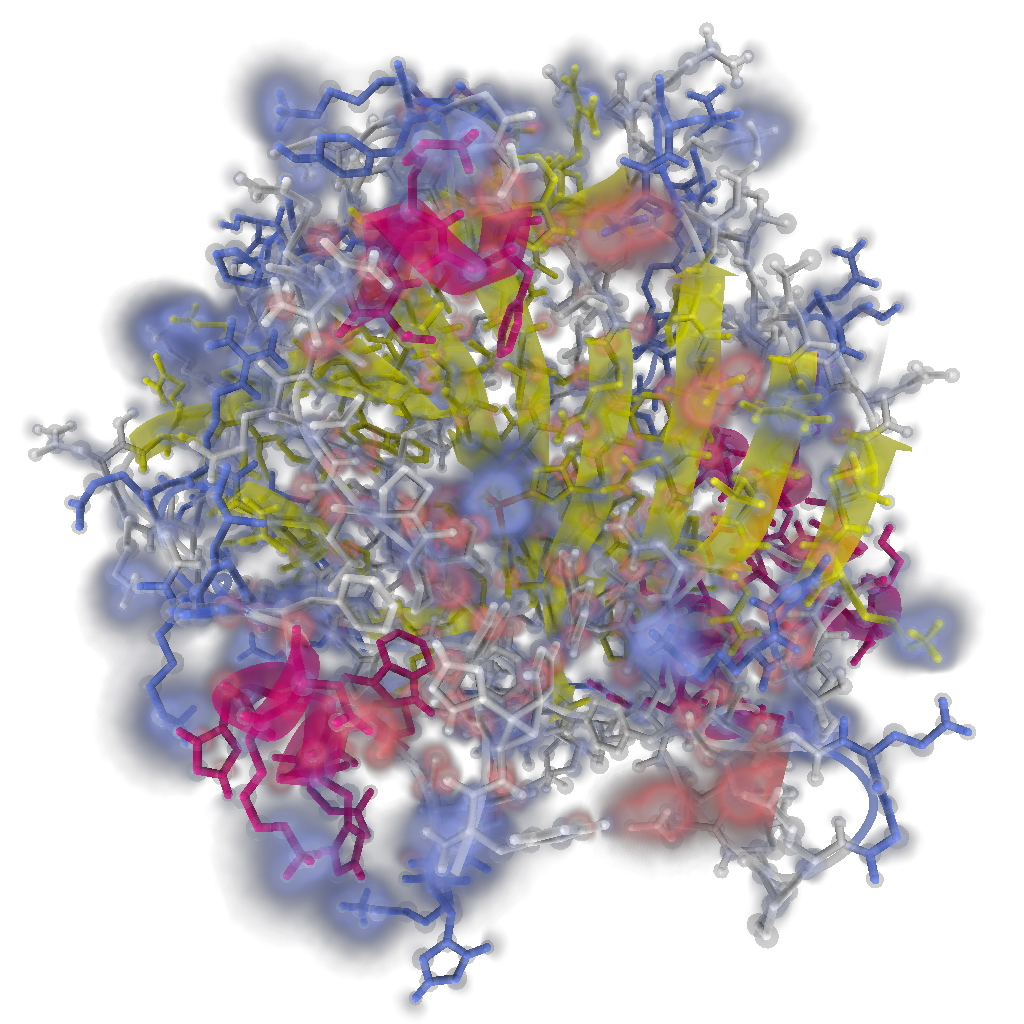
\includegraphics[width=\linewidth]{snapshots/mol/cgf/render.jpg}%
      \subcaption{\label{fig:sub:protein}%
        hybrid visualization
      }%
    \end{minipage}%
  }
  \settoheight{\boxheight}{\usebox\savedProteinBox}
  % 
	\hspace*{\fill}%
  \begin{minipage}[b][\boxheight][b]{0.24\linewidth}
    \centering%
    \begin{minipage}[t]{0.98\linewidth}
      \centering
      \setlength{\imgWidth}{\textwidth}
      \splitImage{snapshots/mol/cgf/g1.jpg}{snapshots/mol/cgf/g2.jpg}\vspace{-4mm}
      \subcaption{\label{fig:sub:protein-geoms}%
        geometric data
      }
    \end{minipage}%
    \vfill%
    \begin{minipage}[b]{0.98\linewidth}
      \centering
      % 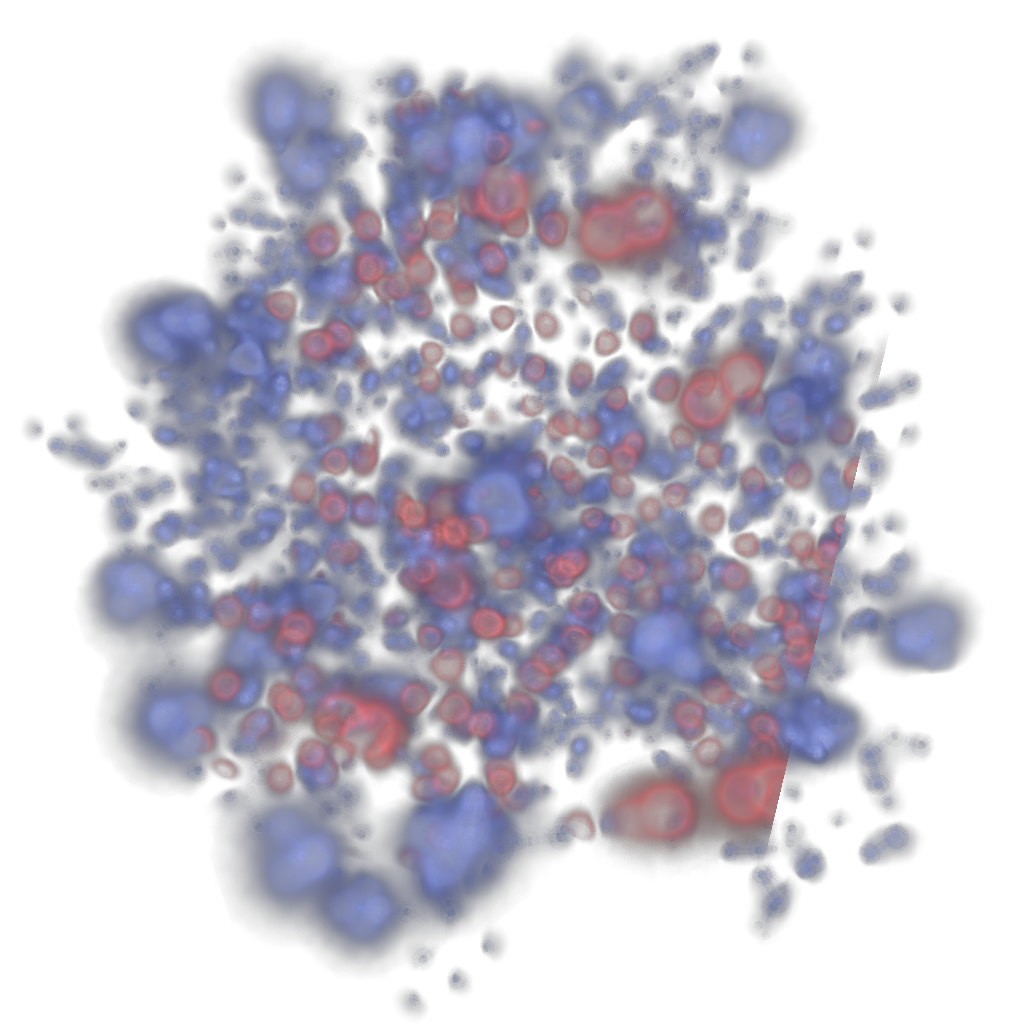
\includegraphics[width=0.98\linewidth]{snapshots/mol/cgf/vols}
      \setlength{\imgWidth}{\textwidth}
      \splitImage{snapshots/mol/cgf/v1.jpg}{snapshots/mol/cgf/v2.jpg}\vspace{-4mm}
      \subcaption{\label{fig:sub:protein-vols}%
        volume data
      }
    \end{minipage}%
  \end{minipage}%
  \hfill%
  %% central image
  \usebox\savedProteinBox
  \hfill%
  \begin{minipage}[b][\boxheight][b]{0.24\linewidth}
    \centering%
    \begin{minipage}[t]{0.98\linewidth}
      \centering
      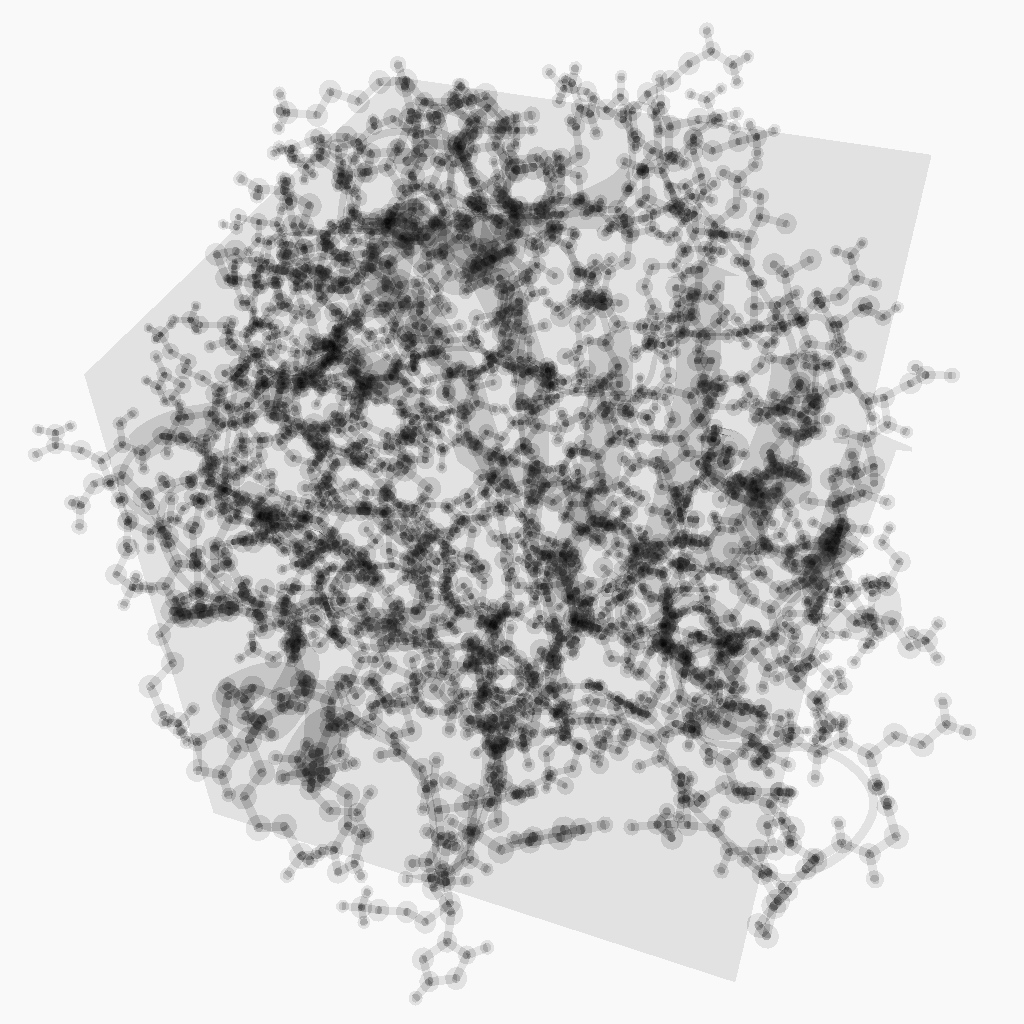
\includegraphics[width=\linewidth]{snapshots/mol/cgf/dci-scaled-inv.jpg}
      \subcaption{\label{fig:sub:protein-dci}%
        depth complexity
      }
    \end{minipage}%
    \vfill%
    \begin{minipage}[b]{0.98\linewidth}
      \centering
     %\includegraphics[width=\linewidth]{snapshots/mol/cgf/dch-64-max46}
      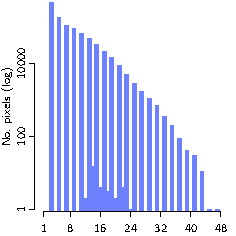
\includegraphics[width=1\linewidth]{figures/plot-dch-mol}\vspace{-2mm}
      \subcaption{\label{fig:sub:protein-dch}%
        \dch{} (log scale)%depth complexity histogram
      }
    \end{minipage}%
  \end{minipage}%
	\hspace*{\fill}%
  % 
  \caption{\label{fig:protein}%
    Visualization of a protein (\emph{human carbonic anhydrase II}) combining hybrid data from different sources.
    (\subref{fig:sub:protein})~final rendering of hybrid visualization.
    (\subref{fig:sub:protein-geoms})~geometric protein representations. 
    (\subref{fig:sub:protein-vols})~volumetric data sources depicting electrostatic potentials. 
    (\subref{fig:sub:protein-dci})~image-space depth complexity (re-scaled for representational purposes). 
    (\subref{fig:sub:protein-dch})~depth complexity histogram (DCH, log scale). %% showing a maximum of $46$ depth layers. 
    Our improved \ab{} algorithm is capable of rendering the entire scene at 32\,fps---a performance increase of $5.9$ times compared to prevalent techniques. %perfnumber
  }
\end{figure*}



\section{Visualization of Scenes with Non-uniform Depth Complexity}
\label{sec:depthcomplexity}

In this paper, we have chosen four representative scenes of different fields including molecular science (\emph{protein}), space weather simulations (\emph{space}), neurosurgical treatment planning (\emph{medical}), and computational fluid dynamics (\emph{cfd}). 
Characteristic for the selected scenes is that the major computational costs arise from the task of ordering all contributions in terms of visibility. 
In modern OIT solutions, these costs are directly related to the observed depth complexity in the image, i.e., the number of overlapping contributions per pixel. 
At the same time, most scenes often feature non-uniform complexity distributions in image space with clusters of high depth complexity surrounded by regions of lower complexity. 

% Molecular
%
The first hybrid data scene is shown in Figure~\ref{fig:protein} and depicts the protein \emph{human carbonic anhydrase II} (PDB-ID: 2CBA). 
The scene contains protein structures stored in polygonal meshes and volumetric data sources representing electron charge densities. 
Such protein visualizations are commonly used to examine possible docking positions between the protein and other molecules~\cite{Seeliger2010}. 
%
To analyze the complexity of such scenes we thus utilize depth complexity histograms.

\subsection{Depth Complexity Histograms}
\label{sec:dch}
   
As an example for the Depth Complexity Histogram (\dch), we use the protein scene in Figure~\ref{fig:protein}, where the DCH for the shown camera setting is depicted in (\subref{fig:sub:protein-dch}). 
The \dch{} is computed by first rendering a depth complexity image as shown in (\subref{fig:sub:protein-dci}) (note that the image shown has been normalized and inverted for presentational purposes). 
When rendering the complexity image, both shading and blending are disabled. 
All geometries and volume bounding boxes are rendered into an integer image aligned with the current viewport. 
The pixels of this image act as atomic counters and are incremented by the incoming fragments. 
Each pixel of the complexity image thus holds the number of fragments. 
The \dch{} is then computed as a standard histogram over this integer image. 
Each bin in a \dch{} is thereby associated with a complexity range and holds the number of pixels whose depth complexities fall within that range. 

\begin{figure}[t]
  \centering
  \begin{minipage}{1.0\linewidth}\centering
    \fbox{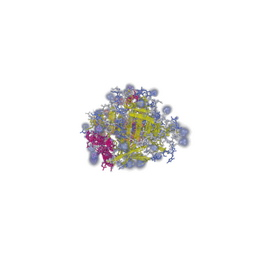
\includegraphics[width=0.16\linewidth]{snapshots/mol/cgf/viewdep/0050_resize.jpg}}%
    \hfill%
    \fbox{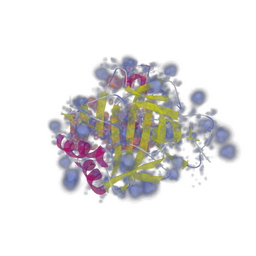
\includegraphics[width=0.16\linewidth]{snapshots/mol/cgf/viewdep/0150_resize.jpg}}%
    \hfill%
    \fbox{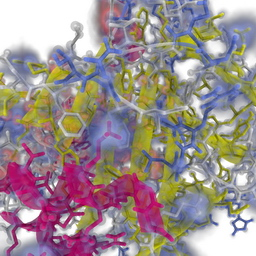
\includegraphics[width=0.16\linewidth]{snapshots/mol/cgf/viewdep/0250_resize.jpg}}%
    \hfill%
    \fbox{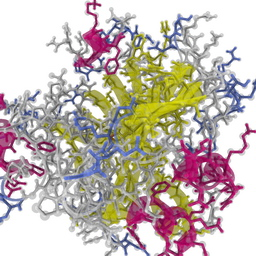
\includegraphics[width=0.16\linewidth]{snapshots/mol/cgf/viewdep/0350_resize.jpg}}%
    \hfill%
    \fbox{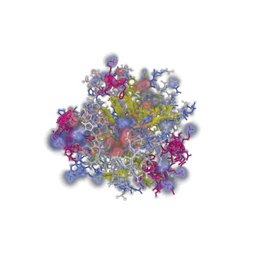
\includegraphics[width=0.16\linewidth]{snapshots/mol/cgf/viewdep/0450_resize.jpg}}%
    \hspace{9mm}
  \end{minipage}\\
  % 
  \begin{minipage}{1.0\linewidth}\centering
    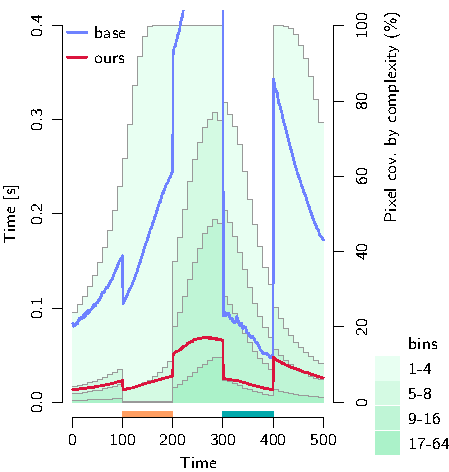
\includegraphics[width=\linewidth]{figures/plot-viewdep-tall} 
  \end{minipage}
  % 
  \caption{\label{fig:viewdep}%
    Performance and complexity over time for a predefined camera path around the protein data set of Figure~\ref{fig:protein}. 
    Rendering times are shown as lines (first y-axis) and \dch{}s as bar charts (second y-axis). 
    The camera dollies in and out while the scene composition is changed every $100\textsuperscript{th}$ step. 
  }
\end{figure}



\subsection{Visualization Challenges for Data Fusion}
\label{sec:vischallenges}

During the analysis of our four scenes, we made the observation that many pixels feature a low depth complexity and only a few pixels feature the highest depth complexities. 
This results in rapidly decreasing \dch{}s where the majority of pixels have a complexity that is only a fraction of the global maximum of the scene.
In our experience, these findings are also applicable to many other scenes.

Again, we use the protein scene in Figure~\ref{fig:protein} as an example. 
From a depth complexity perspective, the protein scene is fairly well behaved.
The maximum depth complexity is limited and the points with high depth complexity are evenly distributed across the entire scene. 
The \dch{}, however, decreases rapidly.
Note that the \dch{} in Figure~\ref{fig:protein}(\subref{fig:sub:protein-dch}) is plotted logarithmically.
The dominance of even-numbered depth complexities is a result of closed geometries. 
The majority of all pixels ($68\,\%$) have a depth complexity of 8 or less, whereas only very few pixels ($6.6\,\%$) have a complexity larger than 17 with a maximum of 46 for this specific camera setting. 

\dch{}s are not only dependent on scene content but also on the camera settings.
Figure~\ref{fig:viewdep} illustrates how the \dch{} changes for the protein scene for an animated camera path.
The time-dependent \dch{}s are shown as vertical bar-plots of screen coverage in percent (linear scale, right y-axis).
Complexities have been binned according to the legend in the lower right and the \dch{} is plotted for every tenth time step.
The camera path is illustrated with five snapshots taken at time points 50, 150, 250, 350, and 450 respectively (top row of images).
Additionally, the figure also shows performance (red and blue line plots, left y-axis) which will be discussed in later sections.
%
In addition to camera movement, the scene composition is changed every $100\textsuperscript{th}$ time-point.
%% from caption
At the first marker (orange), the geometry of the stick representation is removed (cf.~Figure~\ref{fig:protein}(\subref{fig:sub:protein-geoms})) reducing high-complexity pixels. 
At the second marker (green), both volume data sources are removed (cf.~Figure~\ref{fig:protein}(\subref{fig:sub:protein-vols})) reducing low-complexity pixels. 
From the plots, we can see that the \dch{} changes over time and that the rendering performance depend on these changes.
We can also see that the \dch{} remains non-uniform in nature even with the camera very close to the protein.
This opens up the possibility to save resources if the memory allocation could be adapted to the observed complexity on a per pixel basis.
In the next section we provide a technical description of how current state-of-the-art OIT techniques adapt to non-uniform scene complexities. 


\newcommand{\bFraglist}{Fragment List}

\newcommand{\bTarget}{Render Target}
\newcommand{\bAnchor}{List Anchor}
\newcommand{\bPool}{Fragment Pool}
\newcommand{\bAtomic}{Atomic}
\newcommand{\bSemaphore}{Semaphore}
\newcommand{\bArray}{Local Array}
\newcommand{\bCounter}{Complexity Counter}

\newcommand{\sClear}{Clear Step}
\newcommand{\sFill}{Fill Step}
\newcommand{\sResolve}{Resolve Step}

\newcommand{\sCount}{Count Step}
\newcommand{\sSegment}{Segmentation Step}
\newcommand{\sTrigger}{Per-Segment Resolve}

\newcommand{\las}{L} %Local Array Size
\newcommand{\abs}{ABuffer\_frag}







\begin{figure}[t]
  \centering
    %\def\svgwidth{\linewidth}%
    \graphicspath{{figures/}}%
    %% change font within next curly braces, e.g. \sffamily\footnotesize
    {\sffamily\footnotesize\input{figures/abuffer-flowchart.pdf_tex}}
    %
  \caption{\label{fig:abuffer-flowchart}% 
	Overview of the \ab{} rendering approach on GPU hardware. 
	Previous work has primarily focused on global memory management during the \sFill. 
	Our proposed algorithm is hence aimed at local GPU cache memory. 
	Memory related steps are highlighted in blue.
   }
\end{figure}


\section{Algorithms for Semi-Transparent Data Fusion}
\label{sec:oit-global}

To construct an optimized algorithm we exploit the trend of non-uniform \dch{}s observed earlier.
Three state-of-the-art implementations of the \ab{} concept serve as a reference.
This section details the differences of those algorithms in the dynamic management of {global} GPU memory.
In addition, we show how to further optimize the algorithms with respect to their use of {local} caches on modern graphics hardware.

\begin{figure*}[t]
  \centering
    \def\svgwidth{\textwidth}%
    \graphicspath{{figures/}}%
    %% change font within next curly braces, e.g. \sffamily\footnotesize
    {\sffamily\footnotesize\input{figures/algorithm-overview.pdf_tex}}
    %
  \caption{\label{fig:abuffer-global}%
    Comparison of three existing \ab{} implementations for managing global GPU memory. 
    Both, the DFB and PPLL approaches adapt well to scenes with non-uniform depth complexities by allowing dynamic memory utilization. 
  }
\end{figure*}


The principle of the \ab{} is to capture and store a list of rasterized fragments on a per-pixel basis (called \emph{\bFraglist}). 
This involves three sequential steps as illustrated in Figure~\ref{fig:abuffer-flowchart}: the \sClear, the \sFill, and the \sResolve. 
Both the \sFill{} and \sResolve{} contain sub-steps associated with memory management (highlighted in blue). 
This includes global memory management mainly during the \sFill{} and local cache management in the \sResolve.
Fragment data structure and further considerations on source types will be described in Section~\ref{sec:fusion}.





\subsubsection*{Managing Global GPU Memory}

Three prevalent approaches for managing the global \ab{} memory during the \sFill{} are used.
These are Fixed Fragment Buffers (FFB)~\cite{Crassin2010}, Dynamic Fragment Buffers (DFB)~\cite{Maule2012,Vasilakis2012}, and Per-Pixel Linked Lists (PPLL) \cite{kainz2009ray,Yang2010,Crassin2010}. 

In Figure~\ref{fig:abuffer-global}, the three approaches are illustrated side-by-side.  
In each approach, every pixel is associated with a fragment counter and an implicit or explicit pointer to the stored \bFraglist. 
For the FFB, the global memory pool is statically partitioned and the pointer is implicitly given by the screen coordinates of the fragments. 
The global memory pool of the DFB is dynamically partitioned each frame and the explicit pointer holds a base offset into the pool. 
For the PPLL, the pointer denotes the list anchor for a linked list of fragments spread throughout the pool. 
Both, FFB and DFB ensure a contiguous memory layout for each individual pixel. 
The \bFraglist s are generally stored out-of-order in the comparatively slow but large global memory of the GPU.

DFB and PPLL are both dynamic algorithms and adapt the utilization of global memory well to non-uniform depth complexity distributions. 
Thus, consumption of global memory is almost optimal even for rapidly decreasing \dch{}s. 


\begin{figure*}[t]
  \centering
  \def\svgwidth{\textwidth}%
  \graphicspath{{figures/}}%
  %% change font within next curly braces, e.g. \sffamily\footnotesize
  {\sffamily\footnotesize\input{figures/algorithm-optimization.pdf_tex}}
  % 
  \caption{\label{fig:abuffer-local} %
    Comparison of approaches managing local GPU caches: static management (left) and our two proposed components \stencil{} (center) and \dloop{} (right).
    The unsorted input \bFraglist{} (top) corresponds to the output of the \sFill{} and resides in global memory. 
    The array is sorted in local caches during the \sResolve{} using predefined array sizes. 
    Two pixels are exemplified, a heavy pixel (blue) and a light pixel (orange). 
    The \stencil{} component significantly lowers the amount of unused memory (shown in gray), while the \dloop{} component lowers the amount of both unused and used memory by recycling it.
  }
\end{figure*}


\subsubsection*{Managing Local GPU Caches}

It is common practice to avoid the higher latency of global memory by copying the unsorted \bFraglist\ to a local cache before sorting.
An important aspect of such cache utilization is that the memory layout of modern GPUs typically exposes a limited shared cache to a group of cores. 
Additionally, modern GPUs hide global memory latency by hot swapping groups of threads in a manner similar to pipelining on a CPU~\cite{Nvidia2011}. 
Under ideal circumstances, the number of active threads can be eight times higher than the number of physical cores. 
Per thread allocations therefore need to be small enough such that all active threads designated to a group of cores can have their arrays allocated simultaneously. 
It is thus important to minimize the allocation of cache memory to maximize performance. 
Current trends also indicate that the number of cores increases faster than the available shared cache size, potentially escalating this problem in the future. 

The prevalent approach described in the literature for managing local GPU caches is to allocate a fixed sized array, of size $N$ per thread~\cite{Crassin2010,Maule2012}. 
This has two immediate consequences. 
First, the maximum depth complexity handled by the approach is limited to $N$, since all fragments beyond this number are discarded.
Second, larger array sizes significantly reduce the number of active threads due to cache overflow and reduced hot swapping. 
A number often reported in the literature is $N=64$. 
While the literature includes strategies, such as DFB and PPLL, for managing the global memory, there still remains room for improvement in managing local caches.


\section{Improved Dynamic Depth Complexity Management}
\label{sec:oit-local}

We propose two novel \ab{} components for \ab{} based algorithms based on the observed nature of the \dch{}s. 
Both components are designed to improve the management of local GPU caches. 
For clarity, we will use the term \bArray{} to indicate the fast (local) memory allocated for the sorting of fragments. 

The first component, illustrated in the center of Figure~\ref{fig:abuffer-local}, is called {per-pixel Array Optimization} (\stencil) and ensures that all pixels are evaluated without allocating excessively large \bArray{}s. 
The component segments image space into sections of similar depth complexity and separate shaders, compiled with different local arrays sizes, are triggered for each segment. 
The second component, illustrated to the right in Figure~\ref{fig:abuffer-local}, is part of the \sResolve\ and corresponds to a novel sorting procedure called per-pixel Depth Peeling (\dloop).
The component breaks the sorting into smaller pieces by not loading all fragments at once and can thereby recycle memory. 

A key factor of both components is that they are designed to be used in combination with the current state-of-the-art management of global memory described in the previous section. 
The full rendering algorithm, optimized for geometry intensive fusion scenes, is thus formed by combining the components proposed here with one of the existing solutions for global management, such as DFB or PPLL. 


\subsection{Dynamic Resource Management Using per-pixel Array Optimization}
\label{sec:ppao}

The objective of the proposed \stencil{} component is to limit the amount of unused memory in the local cache by performing the \sResolve{} with \bArray{}s that better correspond to the depth complexity of individual pixels. 
Due to restrictions in GPU cache allocations, the optimization of per-pixel array sizes requires multiple shader programs to be instantiated for different \bArray{} sizes.
Rather than using a unique shader for every possible \bArray{} size we use a smaller set of pre-defined array sizes. 
This leads to a clustering of pixels with similar depth complexity into segments. 
All pixels in a segment are then resolved in a batch by a single shader. 
The full image is then processed in as many batches as there are segments. 
Note that the clustering is independent of the actual pixel locations and that each segment not necessarily corresponds to a focused region in the image. 
The \stencil{} is positioned after the \sFill{} in the \ab{} algorithm (cf.~Figure~\ref{fig:abuffer-flowchart}) making the \stencil{} responsible for managing and calling the \sResolve{} on the respective complexity segments.
The \stencil{} algorithm is outlined below.

%% begingroup/endgroup stuff is necessary for placing the algorithm exactly here ([H]) in two-column mode
\begingroup
\removelatexerror% Nullify \@latex@error
\begin{algorithm}[H]
  %
  %$C \longleftarrow {8, 32, 128}$\; // set of complexity segments
  % count depth complexity $\forall$ pixels during \sFill\;
  \tcp{\sFill}
  \ForAll{pixels of the framebuffer}{ 
    count depth complexity;
  }
  \tcp{\sResolve, loop over all complexity segments}
  \ForEach{$i \in \{8, 16, \dots, \mathrm{max}\}$}{
    activate shader program for complexity segment $i$\;
		\ForAll{unresolved pixels of the framebuffer}{ 
      \tcp{mask pixel if not part of segment class $i$}
      \If{$\mathrm{depth\ complexity}(p) <= i$}{
        resolve segment with \bArray{} of size $i$\;
				\tcp{mark pixel as resolved}
      }
    }
  }
\end{algorithm}
\endgroup

The instantiation procedure of the shader programs is straightforward as the individual instances only differ by a single number (the predetermined buffer size). 
It is also sufficient to instantiate only a small set of shaders due to the decreasing power curve observed in most \dch{}s. 
By analyzing the depth complexity of various scenes, we found that complexity segments of sizes $8$, $16$, $32$, \ldots, $N$ give good results with respect to performance and memory consumption.

To perform \stencil, we need to know the depth complexities of all pixels. 
For this purpose, we utilize a separate integer buffer the size of the framebuffer (one atomic counter per pixel) to count the number of fragments per pixel.
The counting can be combined with the scene rasterization in the \sFill{} and, hence, no additional rendering passes are required.
%
Once the depth complexities are known, the different complexity segments may be processed. 
This is done by looping over all pre-defined sizes of complexity segments and activating the shader program with the respective \bArray{} size. 
The clustering of pixels into complexity classes is handled implicitly during runtime by a masking step where all pixels that are not part of the current segment are discarded. 
Note that the graphics pipeline does not need to be flushed between triggering successive segments and that multiple segments may be evaluated in parallel (even if they are triggered sequentially). 
Figure~\ref{fig:abuffer-local}, center, depicts the utilization of our approach for pixels exhibiting high and low depth complexity.

\subsection{Preventing Over-sized Local Arrays Using per-pixel Depth Peeling}
\label{sec:ppdp}

If the number of fragments inside a \bFraglist{} exceeds the buffer size of the \bArray{} information is usually lost and the final rendering result might feature artifacts.
One impractical solution is to increase the size of the \bArray{}s.
However, large parts of the pre-allocated memory will never be used since typically only a few pixels exhibit a high depth complexity (cf.~Section~\ref{sec:dch} and Figure~\ref{fig:abuffer-local}, left).
To overcome this particular problem, we propose a variation of depth peeling on a per-pixel basis to provide a simple way to correctly deal with overflowing \bArray{}s.
Thus, the maximum supported depth complexity is no longer limited by the size of local memory but instead limited only by the amount of available global memory.
In Figure~\ref{fig:abuffer-local}, right, a \bArray{} size of 8 is used to illustrate our approach for two depth complexities.

The \dloop{} algorithm is outlined below and replaces the \sResolve{} for individual pixels in Figure~\ref{fig:abuffer-flowchart}.

%% begingroup/endgroup stuff is necessary for placing the algorithm exactly here ([H]) in two-column mode
\begingroup 
\removelatexerror% Nullify \@latex@error
\begin{algorithm}[H]
  \def\FragList{fragment list}
  \def\Buffer{buffer} %% local Cache
  \def\MinDepth{min depth}

  \def\State{current state}
  \def\Depth{depth}
  \SetKwInOut{Input}{input}
  \SetKwInOut{Output}{output}
  %
  \Input{list of fragment data per pixel} 

  $n \leftarrow $ sizeof(\bArray{})\;
  create \Buffer{} with $n$ elements\;
  set \MinDepth{} to 0\;
  initialize \State\;
  
  \tcp{\sResolve}
  \Repeat{all fragments $f \in $ \FragList{} are resolved}{%
    \ForEach{fragment $f \in $ \FragList{}}{
      \eIf{\Depth($f$) $\le$ \MinDepth}{
        skip $f$ in current pass\;
      }{
        insert $f$ into \Buffer{} with insertion sort\;
        \tcp{store at most $n$ elements}
				\tcp{drop last element on overflow}
      }
    }
    resolve \Buffer{} considering \State\;
    store \MinDepth{} and state of last \Buffer{} element\;
%    store \State{} of last \Buffer{} element\;
    clear \Buffer\;
  }
\end{algorithm}
\endgroup

The \dloop{} algorithm follows the approach of bucket depth peeling where a larger list is sorted and resolved as a set of smaller sequences but does so fully on the GPU between global and local memory without the need to re-render geometry. 
We split the \sResolve{} into several subpasses which allows for the \bArray{} to be recycled and its size to be reduced. 
With a \bArray{} of size $n$, the process sorts $n-1$ elements in the \bFraglist{} per subpass. 
While looping over the contents of the \bFraglist{}, the $n$ entries with the smallest depth values are chosen and stored in the buffer by using insertion sort.
If a fragment was already processed it will be discarded in the current pass.
After filling the buffer its contents are resolved. 
To ensure consistency between the individual resolve passes, we temporarily store the current state of the rendering, including volume occupancy and ray position.
The current state and minimal depth are updated and the local buffer is emptied for the next pass. 
This approach does not require additional rendering passes but does require the entire \bFraglist{} to be read multiple times from global GPU memory. 

Sorting the full array thus takes a maximum of $\left\lceil D/(n-1)\right\rceil$ passes for a pixel with depth complexity $D$. 
The loop may be terminated sooner, e.g.{} in case of early-ray termination, and further read/write intensive sorting operations are avoided. 
Note that the size of the \bArray{} is constant. 
We observed an optimal \bArray{} size of $8$ for our \dloop{} approach across all test setups with respect to performance. 

Note that our \dloop{} algorithm may exhibit z-fighting issues similar to regular depth peeling. 
The issue arises when multiple fragments of a single pixel have identical depth and only a subset of these fragments gets included in one loop iteration. 
Since only the minimal depth is used to distinguish processed fragments from fragments yet to be resolved, the solution is not unique.
This also complicates the decision in the subsequent iterations regarding which fragments should be discarded.
So far in our work we have not experienced any artifacts from this kind of z-fighting. 
Potential solutions exist int he form of additional per-fragment flags which could be used to asses process status at the cost of additional read/write operations. 
A comprehensive discussion on the phenomenon and its solutions can be found in the work of Vasilakis and Fudos~\cite{Vasilakis2013}. 

\section{Fused Rendering of Hybrid Data Sources}
\label{sec:fusion}

So far we have discussed the memory management of the \ab{} involved in the construction of the sorted \bFraglist{} (Figure~\ref{fig:abuffer-flowchart}, blue highlights). 
In this section, we will focus on the \ab{} evaluation and the rendering of the scene (Figure~\ref{fig:abuffer-flowchart}, orange highlight) and implementation details including data structures.

\newcommand{\ccz}{\emph{z}}
\newcommand{\ccid}{\emph{id}}
\newcommand{\cccol}{\emph{color}}

\subsection{\bFraglist{} Creation and Evaluation}

The following data structure is used for all fragments generated in the \sFill\ as entries of the \bFraglist: 
\ccz{} (float32), \ccid{} (int32), \cccol{} (vec4 float16).
The structure has a total size of 16 bytes and the same data structure is used for both geometric and volumetric contributions. 

In the \sFill, \abs{} entries are computed and stored in the \bFraglist. 
Geometric sources are shaded during this step and the computed color is stored explicitly in the \cccol{} component. 
For volumetric sources, only the associated proxy geometry is rendered during the \sFill{} and the \cccol{} component is left uninitialized. 
The \ccz{} and \ccid{} components are treated identically for all source types and respectively hold the depth value in screen space coordinates and a unique source identifier. 
Bit operations are used on the \ccid{} component to store both source type as well as a unique identifier. 
Sources may be rendered independently by different shaders but the produced fragments (instances of \abs) are all inserted into the same global storage.

During the final stage of the \sResolve, the scene content is evaluated and blended into the framebuffer. 
At this point, all entries in the \bFraglist{} can be interpreted as intersection points along the view rays. 
Ray casting of the scene is performed in world space by sequentially looping over all entries in the \bFraglist. 
Geometry fragments are blended directly to the buffer while volume rendering is performed for the interleaved ray segments. 
Volume occupancy is tracked through a bitmask which is updated every time a fragment of a volume proxy geometry is encountered. 
For more information on fragment list evaluation, particularly the use of bitmasks to track volume occupancy, we direct the reader to Brecheisen \etal{}~\cite{brecheisen08multimodal}. 
Once the occupancy and entry and exit points are known, the problem is reduced to the problem of multi-volume rendering as discussed in Section~\ref{sec:related-work}. 


\subsection{Implementation Details}

Our implementation supports global memory management using FFB, DFB, and PPLL as described in Section~\ref{sec:oit-global}. 
The FFB and PPLL implementations are derived from the work by Crassin~\cite{Crassin2010}.
The code for the DFB implementation was provided by Maule~\etal \cite{Maule2012} and was slightly changed to fit our needs.
We use C++, OpenGL, and GLSL for our framework.
The only exception is the scan step of the DFB implementation which is performed in CUDA using the CUDA Thrust library as explained by Maule~\etal

For management of local cache memory we utilize our proposed components: \stencil{} and \dloop{} (cf.~Section~\ref{sec:oit-local}). 
The \stencil{} component is implemented using an 8bit stencil buffer for masking the different complexity segments to be triggered by separate shaders.  
The \sFill{} is enclosed in a loop on the CPU, where different segments are triggered by modifying the OpenGL stencil function. 
Note that using an $8$bit buffer does not limit the depth complexity to $255$.
Higher complexities are still possible but they will all be associated with the same segment. 
If larger segment limits are needed, the stencil buffer can easily be replaced with a texture of higher precision. 
The \dloop{} approach simply replaces the final steps of the \sResolve{} and the loop is implemented directly in GLSL. 

\bArray{}s are always allocated as local buffers with predefined sizes inside the shaders and are, thus, not assigned explicitly to specific memory. 
Thread scheduling and memory assignment is therefore up to the discretion of the driver.
The entire algorithm, with global and local optimizations, requires the implementation of three shaders namely clear, fill, resolve plus additional clones of the resolve shader containing different buffer sizes for the \stencil{}.




\section{Results}
\label{sec:results}

We tested our proposed \ab{} components with four real-world cases from different fields.
The performance was measured for a viewport size of $1024 \times 768$ on four different NVIDIA GeForce GTX GPUs: 
560, 580, 670, and Titan ($1$\,GiB, $1.5$\,GiB, $2$\,GiB, and $6$\,GiB VRAM respectively).
%
Individual performance for the 580 and Titan are included in the paper (representing Fermi and Kepler architectures respectively). 
Performance for 560 and 670 are available as supplementary material. 
Reported averages were computed across all GPUs. 
Scene configurations will be described next in Section~\ref{sec:scenarios} followed by a presentation of performance in Section~\ref{sec:perf-comp}.

\subsection{Scenario Descriptions}
\label{sec:scenarios}

\begin{description}[font=\normalfont\itshape]
\item[Figure~\ref{fig:protein}, protein:]% 
  The data corresponds to the protein \emph{human carbonic anhydrase II}.
  The scene consists of four separate data sources; two volumetric data sets describing the electrostatic potential calculated at different resolutions and extents, a geometric stick representation of the protein, and a geometric ribbon model of the protein.
  Both geometric representations are colored according to the secondary structure type.
  The three-dimensional structure and potential fields are often visualized to examine potential docking positions between the protein and other molecules \cite{Seeliger2010}.

\item[Figure~\ref{fig:space}, space:]% 
  The space data set depicts results of a multi-variate simulation of a time-dependent 3D magnetohydrodynamics system of the heliosphere during a coronal mass ejection event.
  This particular systems is currently used in space weather prediction \cite{Xie2004}.
  The scene consists of two volumes, showing the number of charged particles and the energy density, and three isosurfaces derived from the energy densities.

\item[Figure~\ref{fig:neuro}, medical:]% 1041 + 637 pathways
  The data, provided as the IEEE Visualization Contest in 2010, contains multiple medical imaging modalities as well as derived information sources for planning neurosurgical intervention~\cite{VisContest2010}.
  The scene consists of four data sources; two volumetric data sets depicting T1-weighted MR images of head and brain, two sources of geometric information in a surface extraction of a tumor segmentation and about $1678$ fiber tracts obtained with diffusion tensor imaging. 
  The combined information from all data sources is used to plan the safest possible access path for an intervention.

\item[Figure~\ref{fig:flow}, cfd:]% 1184 + 1023 + 1037 streamlines
  The data results from a computational fluid dynamics simulation of blood flow in the carotid artery of a human subject.
  The scene consists of a single computed tomography image and two sets of geometric primitives.
  A sparse glyph representation and more than 7500 individual streamlines. 
\end{description}

More details on the different data sources of the individual scenes are listed in Table~\ref{tab:data}.
Depth complexities are available as single view \dch{}s in Figures~\ref{fig:protein} (protein), \ref{fig:space} (space), \ref{fig:neuro} (medical), and \ref{fig:flow} (cfd), respectively. 

\begin{table}[t]
  \centering
  \caption{\label{tab:data}%
    Data information for the four selected scenes, including the first frame of the sequence used for performance tests.
  }
  % 
  \begin{tabular}{ p{1.0cm} l  l  l }
    \toprule
    Scene       & Data & Data size & 1\textsuperscript{st} Frame \\
    \midrule
    
    protein     & \small VOL        & \small $127\times127\times127$ &  
    \multirow{4}{*}{\fbox{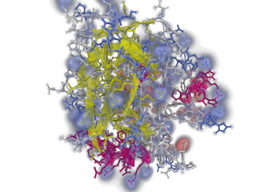
\includegraphics[height=1.2cm]{snapshots/performance/benchimage_Molecule_resize.jpg}}} \\
    & \small VOL        & \small $71\times71\times71$ & \\
    & \small GEO        & \small 868k triangles & \\ % sticks + atoms (454182 + 407040 = 868k)
    & \small GEO        & \small 36k triangles & \\
    \midrule
    
    space       & \small VOL        & \small $256 \times 256 \times 256$ & 
    \multirow{5}{*}{\fbox{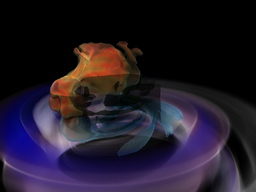
\includegraphics[height=1.2cm]{snapshots/performance/benchimage_Space_resize.jpg}}} \\
    & \small VOL      & \small $256 \times 256 \times 256$ & \\
    & \small GEO        & \small 162k triangles & \\
    & \small GEO        & \small 100k triangles & \\
    & \small GEO        & \small 67k triangles & \\
    \midrule
    
    medical       & \small VOL        & \small $415\times487\times176$ & 
    \multirow{4}{*}{\fbox{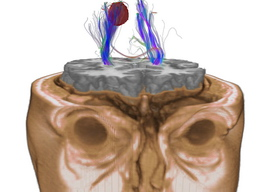
\includegraphics[height=1.2cm]{snapshots/performance/benchimage_Neuro_resize.jpg}}} \\
    & \small VOL        & \small $367\times395\times150$ & \\
    & \small GEO        & \small $363k$ triangles & \\ % tumor (1088617 / 3 = 363k)
    & \small GEO        & \small $1678$ fibers & \\
    \midrule

    cfd        & \small VOL        & \small $76\times49\times45$ & 
    \multirow{4}{*}{\fbox{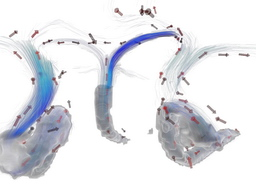
\includegraphics[height=1.2cm]{snapshots/performance/benchimage_Flow_resize.jpg}}} \\
    & \small GEO        & \small $7.5$k streamlines & \\ % 7 x FiberRenderer (~1k each) % 1184 1023 1037 1082 1089 879 1253 = 7547
    & \small GEO        & \small $\approx100$ arrows & \\
    &  &  & \\
    \bottomrule
  \end{tabular}
\end{table}

\subsection{Performance Comparison}
\label{sec:perf-comp}


\begin{figure}[t]
  \centering
    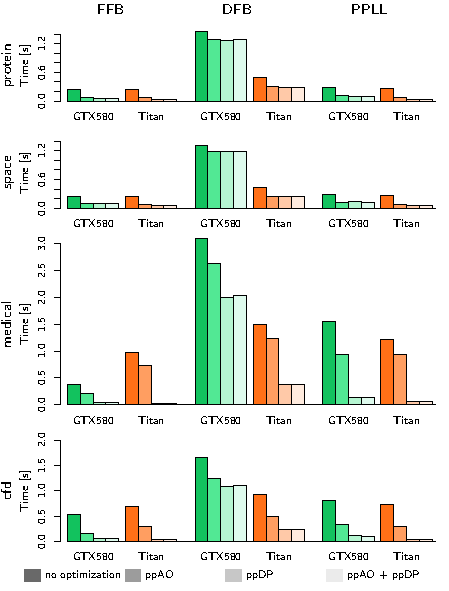
\includegraphics{figures/plot-performance-gtx580} %% width=1.0\linewidth
    \caption{\label{fig:performance}%
      Performance comparison with our proposed \stencil{} and \dloop{} components.
      Columns represent the different \ab{} implementations in combination with our components (none, \stencil{}, \dloop{}, \stencil{} and \dloop{} combined).
    }
\end{figure}


We have investigated how our proposed components improve the performance for each of the three \ab{} algorithms for global memory management. %%Section~\ref{sec:ab-merged}.
For each algorithm, we measured the performance for different combinations.
In Figure~\ref{fig:performance}, the results are shown from top to bottom for the four distinct scenes---protein, space, medical, and cfd.
For each of FFB, DFB, and PPLL, we have measured the performance of four configurations for local memory management; baseline (static buffers), \stencil{}, \dloop{}, and \stencil{}+\dloop{}. 
The largest \bArray{} size allocated for the scenes was set to $64$ (protein), $32$ (space), and $128$ (neuro and flow). 
Allocating a \bArray{} size to hold all depth layers of the medical scene resulted in driver crashes, thus, only the first $128$ layers were resolved for baseline and \stencil{} configurations (\dloop{} is capable of resolving higher complexities with smaller \bArray{}s). 
Likewise, using FFB for global management also limits maximum complexity, requiring approximately $12.6$\,MiB per depth layer at $1024 \times 768$ resolution. 
Depth segments for \stencil{} were chosen as powers of two between $8$ and the scene cap reported above. 
All performance results for \dloop{} were measured with a \bArray{} size set to $8$. 
%% Benchmark results depicted in Figure~\ref{fig:performance} organized by scenes (rows), global algorithms (major columns), and GPUs (minor columns). 
For each test, frame times were computed as the average over $30$ seconds of rendering as the camera rotated around the scene at fixed distance. 
Early-ray termination was enabled for transparency values less than $0.02$ during all benchmarks.

Due to a performance penalty associated with a CUDA/OpenGL context switch, we were unable to achieve results for the DFB on the same level as reported by Maule~\cite{Maule2012}. 
The penalty manifested as a $50\,$ms--$200\,$ms delay associated with the scan step and was persistent across different GPUs and drivers and was also present in a minimal stand-alone DFB implementation.
The results for the DFB approach reported in Figure~\ref{fig:performance} include this penalty.

Supported by the performance graphs, we can say that both \stencil{} and \dloop{} are capable of providing significant performance gains for a large variety of configurations. 
The performance gain is threefold for \stencil{} and about eightfold \dloop{} when averaged over all scenes and GPUs. 
For scenes with high depth complexities or homogeneous depth complexity distributions, the improvement obtained with \stencil{} is reduced since the processing of the heavy pixels becomes a bottleneck. 
In such scenarios, \dloop{} maintains a significant speedup, particularly when early-ray termination is enabled. 

In addition to the four real-world scenarios, we created a synthetic worst-case scene with screen-filling quads.
The scene consists of $64$ quads ($\alpha=0.05$) aligned orthogonal to the viewing direction where their order is randomized in depth. 
The quads are scaled so that they all cover the entire viewport in the middle of the animation.
Thus, all pixels feature a near-maximum depth complexity.
Results are shown in Figure~\ref{fig:viewdep-quad} and confirm that the performance of \stencil{} (as expected) approaches that of statically implemented buffers while \dloop{} maintains a $3.6$ times performance increase. 



\begin{figure}[t]
  \centering
  \begin{minipage}{0.9\linewidth}\centering 
  \begin{minipage}{1.0\linewidth}\centering 
    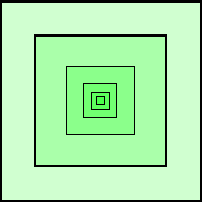
\includegraphics[width=0.14\linewidth]{figures/quads1}\hfill 
    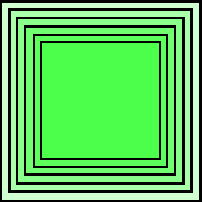
\includegraphics[width=0.14\linewidth]{figures/quads2}\hfill 
    
\includegraphics[width=0.14\linewidth]{figures/quads3}\hfill 
    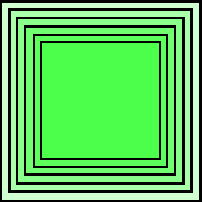
\includegraphics[width=0.14\linewidth]{figures/quads2}\hfill 
    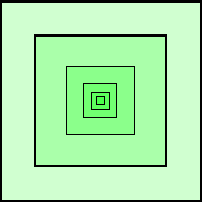
\includegraphics[width=0.14\linewidth]{figures/quads1}\hfill \hspace{6mm}
  \end{minipage}
  % 
  \begin{minipage}{1.0\linewidth}\centering
    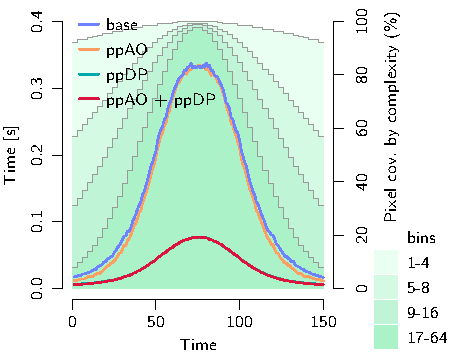
\includegraphics[width=\linewidth]{figures/plot-viewdep-quad-tall} 
  \end{minipage}
  \end{minipage}
  \caption{\label{fig:viewdep-quad}%
    Performance for a synthetic data set.
    Rendering times are shown as lines (first y-axis) and \dch{}s as bar charts (second y-axis). 
  }
\end{figure}


\section{Conclusions and Future Work}
\label{sec:conclusion}


In this paper, we address the challenge of interactive exploration of complex hybrid data. 
Two adaptive data handling components are proposed to be combined with prevalent \ab{} techniques to form a final rendering algorithm. 
Of the two, \dloop{} is better equipped to deal with very high complexities but does so at the cost of potential artifacts from z-fighting while \stencil{} performs well for moderate complexities with exact results. 
Optionally, the components can be combined to achieve support for high depth complexities while guaranteeing a minimum number of correctly blended samples. 

An interesting consequence of our work is the potential alleviation of the traditional trade-off between performance and depth-support. 
We believe that this aspect makes our work valuable also in other areas of visualization or computer graphics that employ \ab{} based techniques.
For example, it may now be possible to encode fiber tracking uncertainties in the alpha channel of the visualized fibers without eliminating the possibility to also visualize a co-registered volume. 



%%% if specified like this the section will be ommitted in review mode
\section*{Acknowledgments}
\label{sec:acknowledgments}
%%
Space simulation data have been provided by CCMC at Goddard Space Flight Center, NASA. 
% the Center for Medical Image  Science and Visualization (CMIV) at Linköping University Sweden and Cyril Crassin.
%%
This work was supported in part by 
the Swedish Research Council, VR grant 2011-5816 and the Linnaeus Environment CADICS, and 
the Swedish e-Science Research Centre (SeRC).

\begin{figure*}[p]
  \centering
  %% 
  %% create final image first to ensure that it is labeled with (a)
  %% do not show it but store it in a box for later use    
  \savebox\savedProteinBox{%
    \begin{minipage}[b]{0.51\linewidth}%
      \centering%
      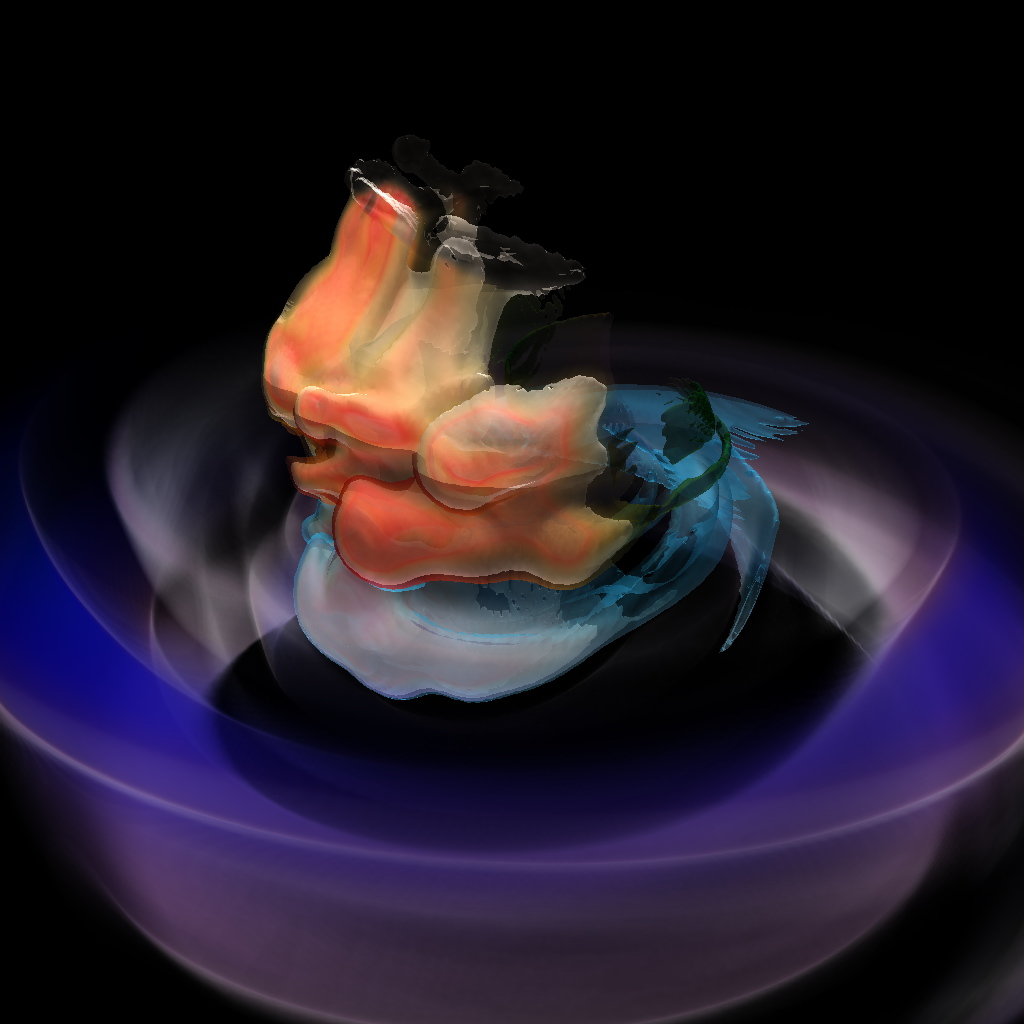
\includegraphics[width=\linewidth]{snapshots/space/space.jpg}%
      \subcaption{\label{fig:sub:space}%
        hybrid visualization
      }%
    \end{minipage}%
  }
  \settoheight{\boxheight}{\usebox\savedProteinBox}
  % 
  \begin{minipage}[b][\boxheight][b]{0.24\linewidth}
    \centering%
    \begin{minipage}[t]{0.98\linewidth}
      \centering
      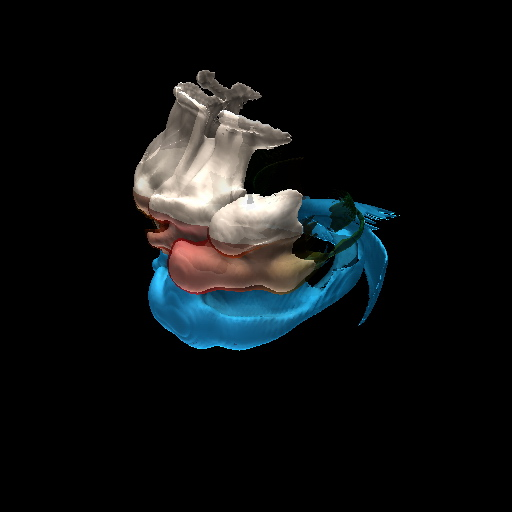
\includegraphics[width=\textwidth]{snapshots/space/space-only-isos.jpg}
      \subcaption{\label{fig:sub:space-geom}%
        geometric data
      }
    \end{minipage}%
    \vfill%
    \begin{minipage}[b]{0.98\linewidth}
      \centering
      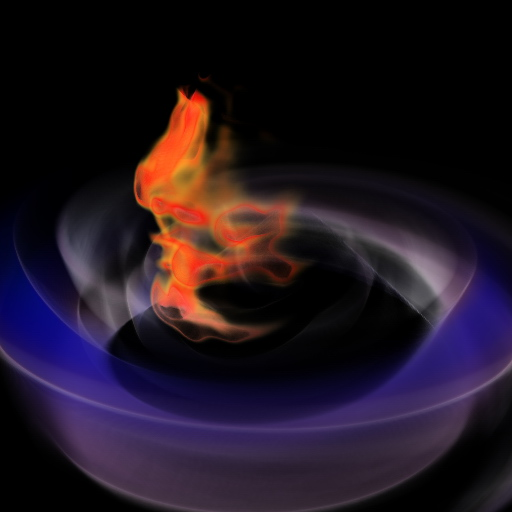
\includegraphics[width=\textwidth]{snapshots/space/space-only-vols.jpg}
      \subcaption{\label{fig:sub:space-vols}%
        volume data
      }
    \end{minipage}%
  \end{minipage}%
  \hfill%
  %% central image
  \usebox\savedProteinBox
  \hfill%
  \begin{minipage}[b][\boxheight][b]{0.24\linewidth}
    \centering%
    \begin{minipage}[t]{0.98\linewidth}
      \centering
      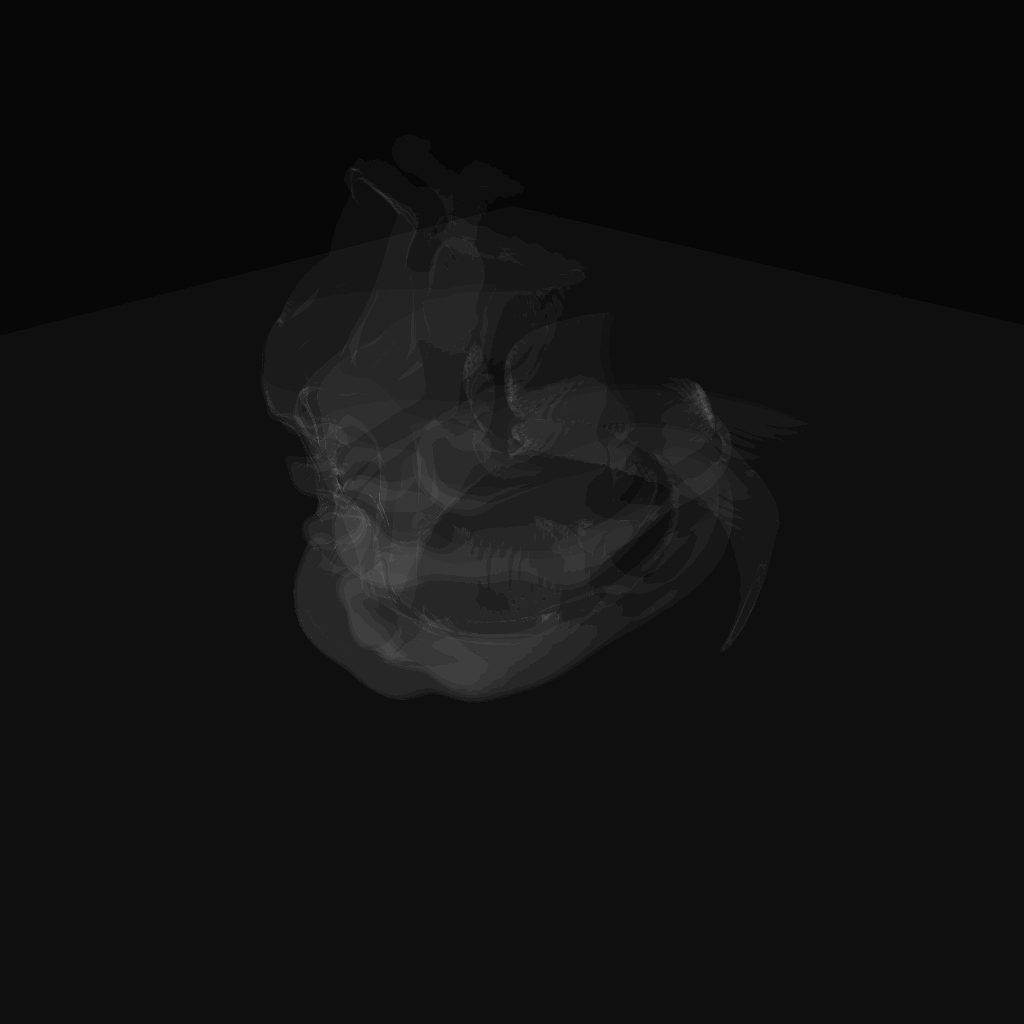
\includegraphics[width=\linewidth]{snapshots/space/space_dci-wp64.jpg}%
      \subcaption{\label{fig:sub:space-dci}%
        depth complexity
      }
    \end{minipage}%
    \vfill%
    \begin{minipage}[b]{0.98\linewidth}
      \centering
      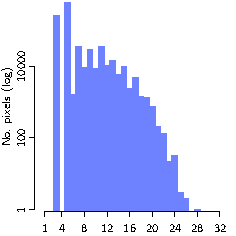
\includegraphics[width=1\linewidth]{figures/plot-dch-space}\vspace{-2mm}
      \subcaption{\label{fig:sub:space-dch}%
        depth complexity histogram
      }
    \end{minipage}%
  \end{minipage}%
  % 
  \caption{\label{fig:space}%
    Visualization of solar mass ejection simulation data used for predicting space weather. 
    (\subref{fig:sub:space})~final rendering of hybrid visualization.
    (\subref{fig:sub:space-geom})~three geometric isosurfaces.
    (\subref*{fig:sub:space-vols})~volumetric data sources. %% depicting inner and outer extents of the simulation at different resolution.
    (\subref{fig:sub:space-dci})~image-space depth complexity (re-scaled for representational purposes). 
    (\subref{fig:sub:space-dch})~depth complexity histogram (DCH, log scale).
    Our improved \ab{} algorithm achieves up to three times the performance compared to existing approaches. %perfnumber
  }
\end{figure*}


\begin{figure*}[p]
  \centering
  \begin{minipage}[b]{0.36\linewidth}\centering
    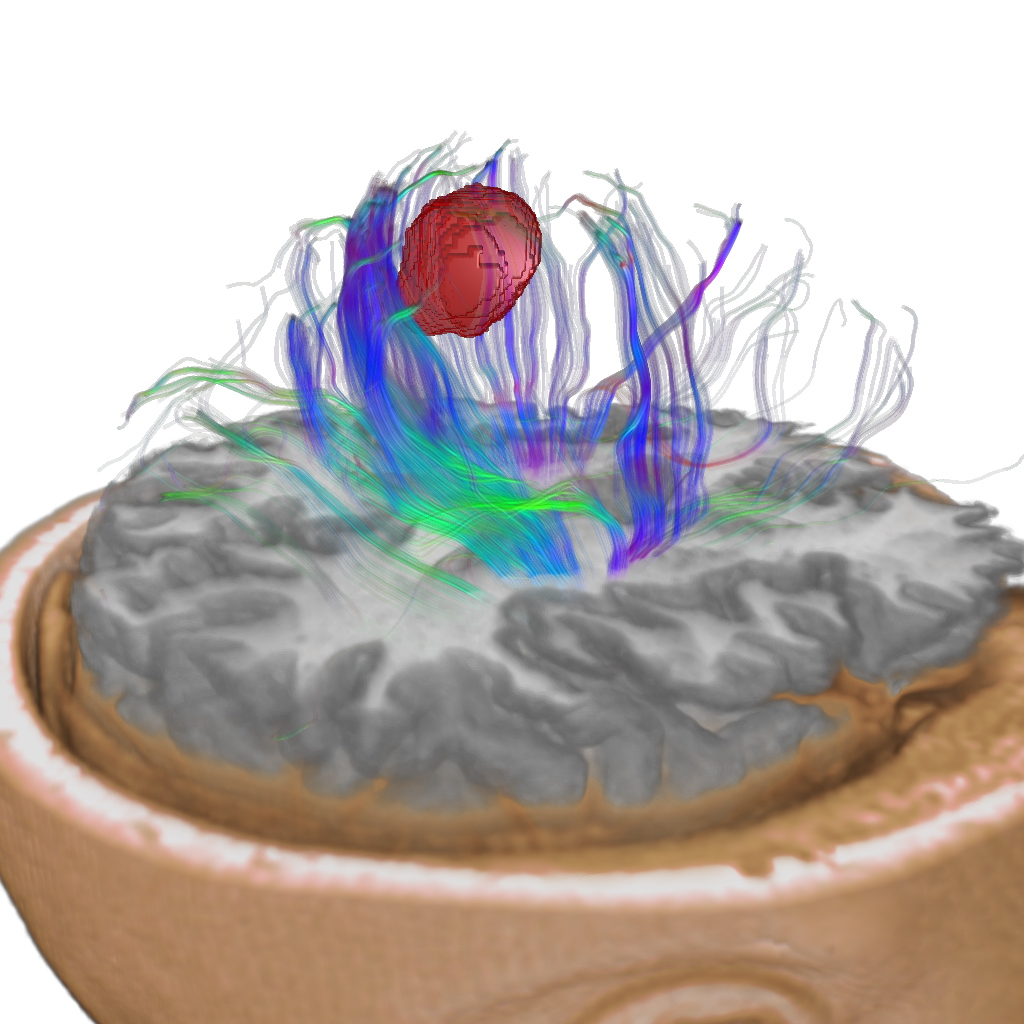
\includegraphics[width=0.98\linewidth]{snapshots/dti/cgf/screenshot_Neuro.jpg}%
    \subcaption{\label{fig:sub:neuro}%
      neurosurgical planning
    }
  \end{minipage}\hfill
  \begin{minipage}[b]{0.36\linewidth}\centering
    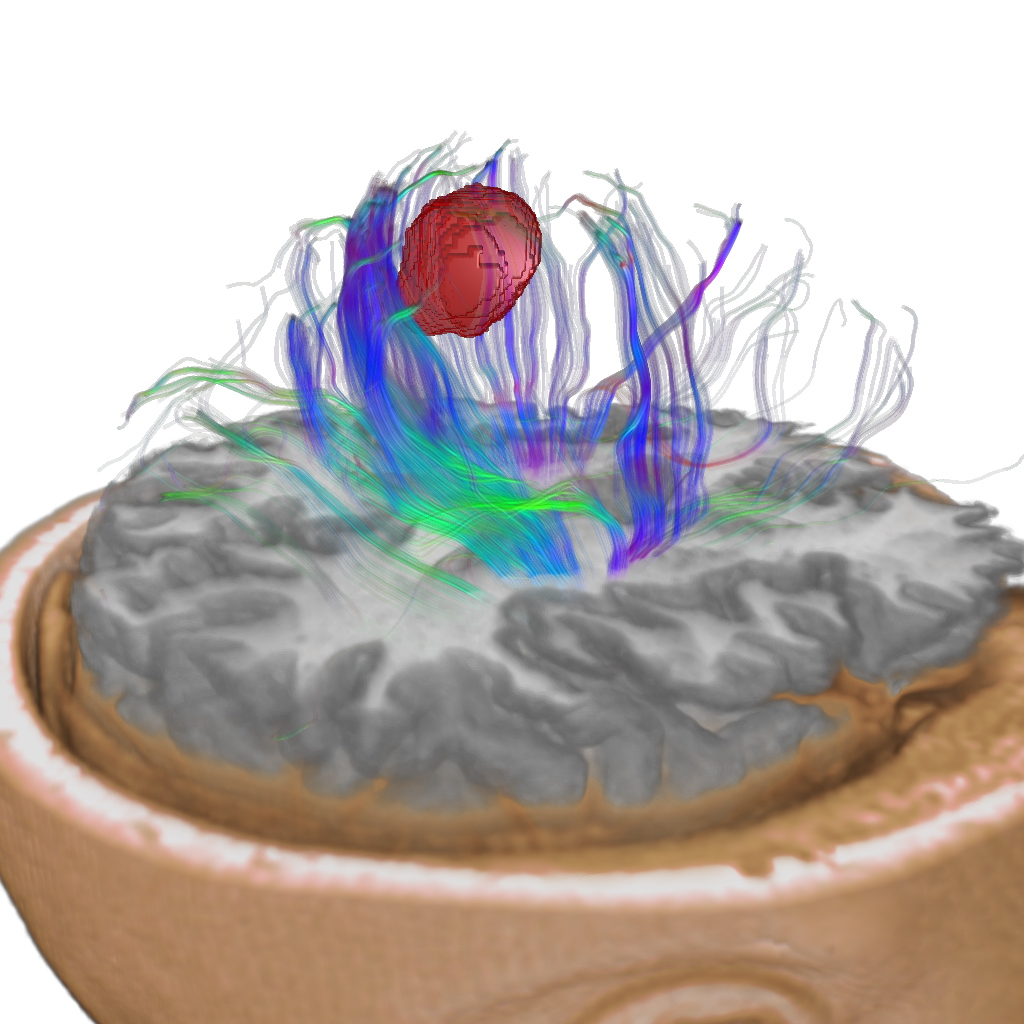
\includegraphics[trim={12cm 15cm 12cm 9cm}, clip, width=0.98\linewidth]{snapshots/dti/cgf/screenshot_Neuro.jpg}%
    \subcaption{\label{fig:sub:neuro-zoom}%
      zoomed view
    }
  \end{minipage}\hfill
  \begin{minipage}[b]{0.26\linewidth}\centering
    % 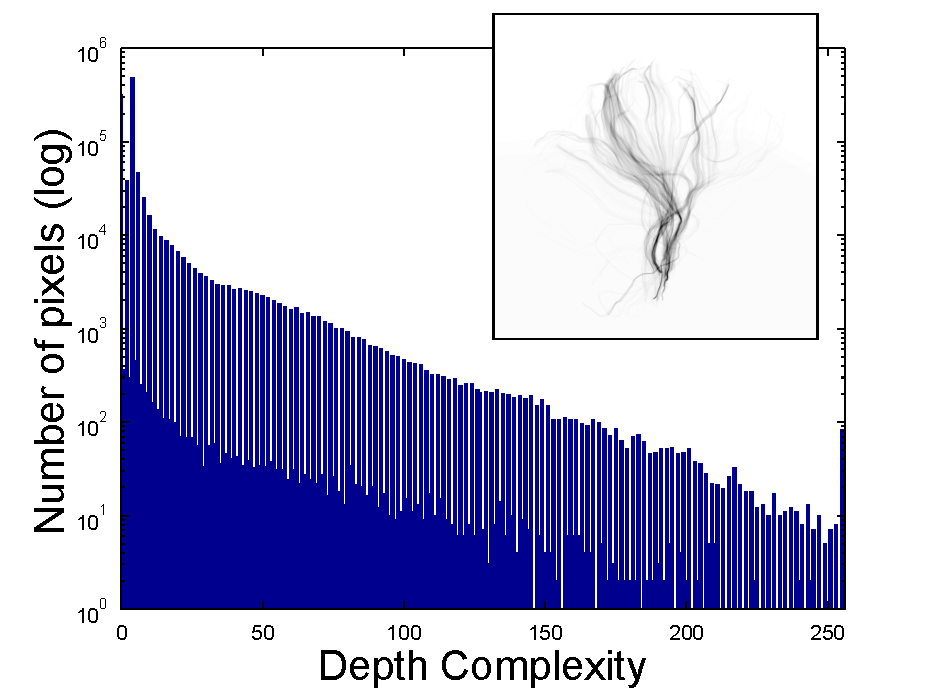
\includegraphics[width=0.98\linewidth]{snapshots/dti/cgf/dci-dch_Neuro_dch-256-max255}
    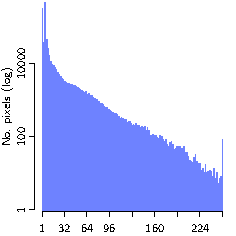
\includegraphics{figures/plot-dch-neuro}
    \subcaption{\label{fig:sub:neuro-dch}%
      \dch{} (log scale)
    }
  \end{minipage}\hfill
  % 
  \caption{\label{fig:neuro}%
    Fused visualization of hybrid data for the purpose of neurosurgical planning.
    The scene is particularly complex in areas where the DTI fibers converge toward two main bundles. 
    (\subref{fig:sub:neuro})~full scene, (\subref{fig:sub:neuro-zoom})~zoomed view, and (\subref{fig:sub:neuro-dch})~the depth complexity histogram (\dch{}, log scale) of~(\subref{fig:sub:neuro}).
  }
\end{figure*}

\begin{figure*}[t]
  \centering
  \begin{minipage}[b]{0.3\linewidth}\centering
    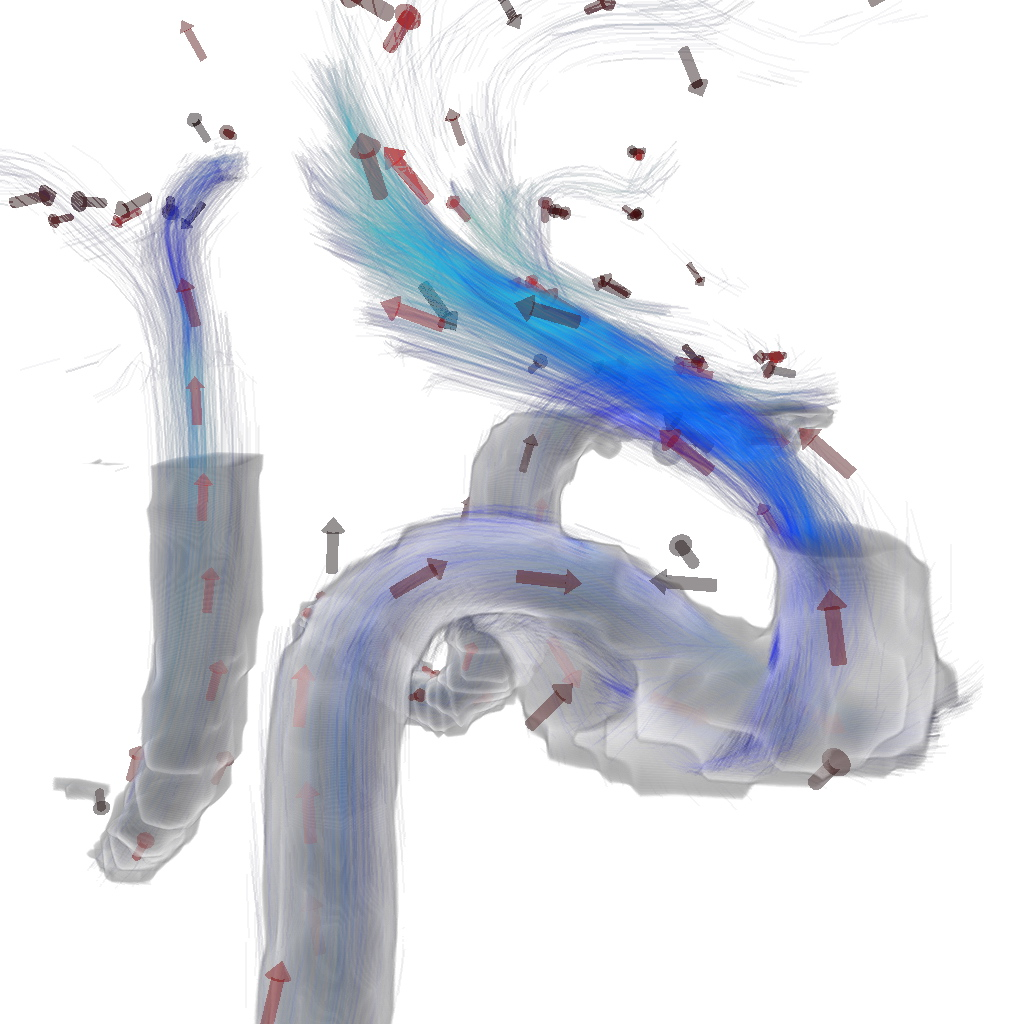
\includegraphics[width=1.0\linewidth]{snapshots/flow/cgf/screenshot_Flow.jpg}
    \subcaption{\label{fig:sub:flow}%
      blood flow
    }
  \end{minipage}\hfill
  \begin{minipage}[b]{0.3\linewidth}\centering
    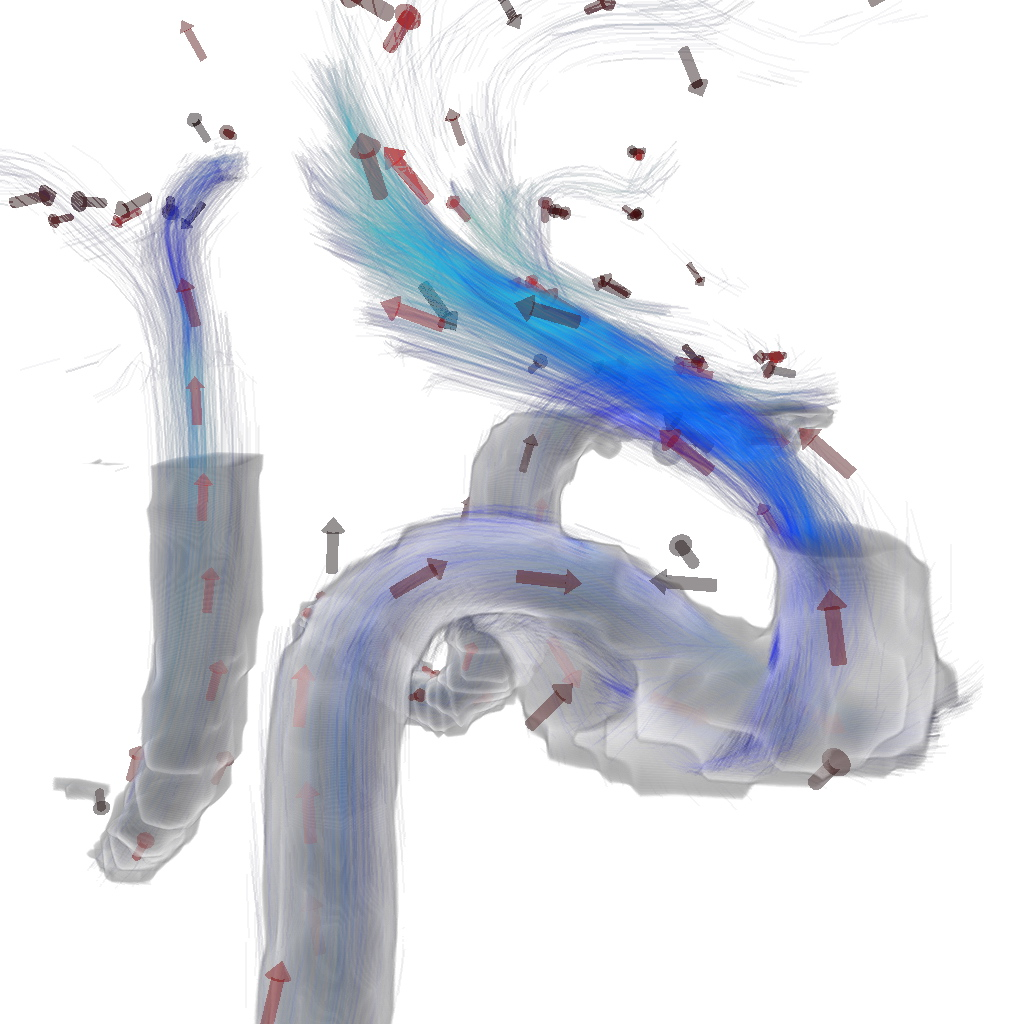
\includegraphics[trim={18cm 16cm 8cm 10cm}, clip, width=1.0\linewidth]{snapshots/flow/cgf/screenshot_Flow.jpg}
    \subcaption{\label{fig:sub:flow-zoom}%
      zoomed view
    }
  \end{minipage}\hfill
  \begin{minipage}[b]{0.26\linewidth}\centering
    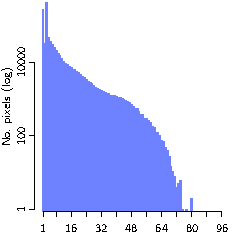
\includegraphics{figures/plot-dch-flow}
    \subcaption{\label{fig:sub:flow-dch}%
      \dch{} (log scale)
    }
  \end{minipage}
  % 
  \caption{\label{fig:flow}%
    Fused visualization of hybrid data used to asses blood flow in the human carotid artery. 
    The rendering uses transparency to reduce the focus on individual streamlines. 
    (\subref{fig:sub:flow})~full scene, (\subref{fig:sub:flow-zoom})~zoomed view, and (\subref{fig:sub:flow-dch})~the depth complexity histogram (\dch{}, log scale) of~(\subref{fig:sub:flow}). %perfnumber
    %% with maximum depth complexities of $294$ (neuro) and $79$ (flow), respectively. 
  }
\end{figure*}


%\bibliographystyle{eg-alpha}
\bibliographystyle{eg-alpha-doi}

\bibliography{literature}

\end{document}




